% Created 2019-06-27 木 15:54
% Intended LaTeX compiler: pdflatex
\documentclass{article}

\usepackage{authblk}
\usepackage{graphicx}
\usepackage{amsfonts}
\usepackage{booktabs}
\usepackage{framed}
\usepackage{xcolor}


\date{} \title{A Series of Graphs With Exponentially Growing
  Reconfigurations Sequences of Independent Sets}
\pagenumbering{gobble}

\author{Volker Turau}
\author{Christoph Weyer}
\affil{Institute of Telematics, Hamburg University of Technology\\ Hamburg, Germany\\ turau@tuhh.de}

\begin{document}
\maketitle

\section{Introduction}
In this note we construct a sequence of graphs $G_c$ with
($c\in \mathbb{N}$) together with two independent sets $S_c$ and $T_c$
such that the shortest reconfiguration sequence between $S_c$ and
$T_c$ grows exponentially with respect to the size of the graphs.
Reconfiguration of independent sets is with respect to the token
jumping rule, i.e., a token can {\em jump} from one node to any other
node as long as the independent set property is retained. In
particular the graph $G_c$ has size $10c$, the independent sets have
size $4c$, and the shortest reconfiguration sequence for $G_c$ has
length $5(3^c-1)$. Table~\ref{tab:length} shows the length of the
sequences for $c=1,5,10$.

\begin{table}[ht]
\centering
\begin{tabular}[t]{c|c}
\toprule
Size of graph&Length of reconfiguration sequence\\
\midrule
10&10\\
50&1210\\
100&295240\\
\bottomrule
\end{tabular}
\caption{Length of reconfiguration sequences for the graphs
  $G_c$.}\label{tab:length}
\end{table}%




\section{The Graph Series $G_{c}$}
The graphs of the sequence we construct are called $G_{c}$ with
$c\in \mathbb{N}$. The basis is the graph $G_{1}$, i.e., $c=1$. This
graph is shown in Fig.~\ref{fig:base_c_1}. The independent set
consists of four nodes depicted in blue, $S_c=\{2,4,7,9\}$ (resp.\
$T_c=\{2,5,7,10\}$) is on the left (resp.\ right). Note that these are
maximum independent sets of $G_1$.

\begin{figure}[ht]
  \begin{minipage}{0.49\textwidth}
    \centering
    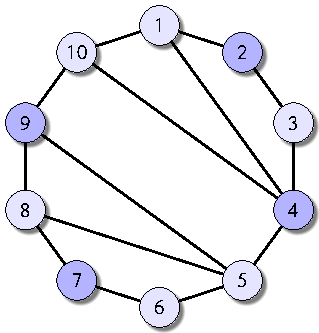
\includegraphics{figures/graph_010_source.pdf}

    Source
  \end{minipage}\hfill
  \begin{minipage}{0.49\textwidth}
    \centering
    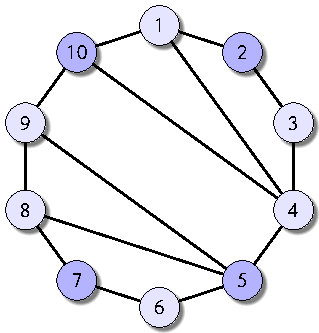
\includegraphics{figures/graph_010_target.pdf}

    Target
  \end{minipage}
  \caption{The base graph $G_{1}$ with 10 nodes. The blue nodes
    depict the start resp.\ the target independent set.}\label{fig:base_c_1}
\end{figure}

Table~\ref{tab:recon1} shows the moves of the shortest reconfiguration
sequence from $S_1$ to $T_1$ in $G_1$, is has length $10$. Note that
$S_1 \cap T_1=\{2,7\}$, i.e., only the tokens of nodes $4$ and $9$
have to be move to $5$ and $10$. None of these moves can be done in
the initial configuration. The first two moves make moving the token
from $4$ to $10$ possible. These moves are rolled back in moves 6 and
7. Moves $4$ and $5$ paved the way to move the token from $9$ to $5$.
These movements are undone in the last two moves. Note that the four
{\em chords} block shorter reconfiguration sequences. Removing either
chord $(4,1)$ or $(5,8)$ would allow a reconfiguration sequence of
length $5$ and removing any of the other two reconfiguration chords
would even allow a length $2$ sequence. Thus, the chords stretch the
shortest reconfiguration sequences. Adding a fifth chord makes a
reconfiguration impossible. The outstanding property of $G_1$ with
respect to $S_1$ is that there is always only one possibility for a
jump, i.e., the corresponding reconfiguration graph is a path.

These observations are the underlying idea of constructing the
sequences of graphs $G_c$. The constructing process consists of two
steps we called {\em duplication} and {\em repetition} process.

\begin{table}[ht]
\centering
\begin{tabular}[t]{c|ll}
\toprule
\#&Independent set & Jump\\
\midrule
&2 4 7 9&\\
1&2 4 6 9& 7 $\rightarrow$ 6\\
2&2 4 6 8& 9 $\rightarrow$ 8\\
3&2 6 8 10& 4 $\rightarrow$ 10\\
4&3 6 8 10& 2 $\rightarrow$ 3\\
5&1 3 6 8& 10 $\rightarrow$ 1\\
6&1 3 6 9& 8 $\rightarrow$ 9\\
7&1 3 7 9& 6 $\rightarrow$ 7\\
8&1 3 5 7& 9 $\rightarrow$ 5\\
9&3 5 7 10& 1 $\rightarrow$ 10\\
10&2 5 7 10& 3 $\rightarrow$ 2\\
\bottomrule
\end{tabular}
\caption{A shortest reconfiguration sequence from $S_1$ to $T_1$ in
  $G_1$ has length $10$.}\label{tab:recon1}
\end{table}%

\section{The Duplication Process}
The duplication process starts by taking two copies of $G_1$. Let
$\hat{G_1}=G_1 \cup \overline{G_1}$, where $\overline{G_1}$ is
isomorphic to $G_1$. The overline operator means that the labels of
the nodes are incremented by $10$, i.e., the nodes of $\overline{G_1}$
are labeled $11,12,\ldots 20$. Note that $\hat{G_1}$ is not
connected. We also construct two independent sets of $\hat{G_1}$:
$\hat{S}_1=S_1 \cup \overline{S_1}$ and
$\hat{T}_1=T_1 \cup \overline{T_1}$.

Since $S_1$ resp.\ $\overline{S_1}$ are maximum independent sets of
$G_1$ resp.\ $\overline{G_1}$ it is impossible to move a token from
$G_1$ to $\overline{G_1}$ or vice versa. Obviously the length of the
shortest reconfiguration sequence from $\hat{S}_1$ to $\hat{T}_1$ in
$\hat{G_1}$ is twice as long as that from $S_1$ to $T_1$ in $G_1$. We
call this reconfiguration sequence the {\em canonical} sequence.

%These are again maximum independent sets of $\hat{G_1}$.

\begin{figure}[ht]
  \centering
  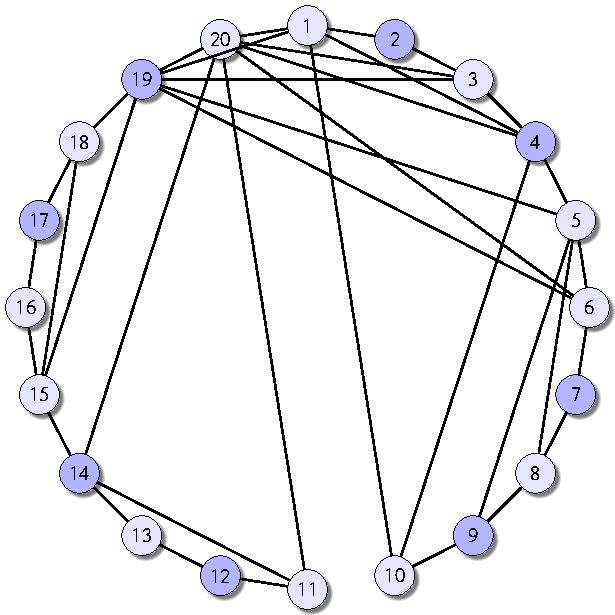
\includegraphics{figures/graph_020.pdf}
  \caption{The graph $G_{2}$ with 20 nodes.}\label{fig:g2}
\end{figure}

In order stretch the reconfiguration sequence from $\hat{S}_1$ to
$\hat{T}_1$ we insert a kind of chords into $\hat{G_1}$, these are
edges from a node in $G_1$ to a node in $\overline{G_1}$. The
intention of inserting these chords is to block the moves of the
canonical sequence.

As stated above a token from $G_1$ (resp.\ $\overline{G_1}$) can only
jump to a node in $G_1$ (resp.\ $\overline{G_1}$). Hence, a
reconfiguration sequence of $\hat{G_1}$ restricted to the nodes of
$G_1$ (resp.\ $\overline{G_1}$) yields a valid reconfiguration
sequence of $G_1$ (resp.\ $\overline{G_1}$). This property remains
true even if we insert chords into $\hat{G_1}$.

The chords are inserted in such a way such that the shortest
reconfiguration sequence $\cal S$ of the resulting graph when
restricted to $G_1$ is equal to original shortest reconfiguration
sequence of the original graph $G_1$, i.e.,
$\left.{\cal S}\right|_{G_1}$ is equal to the reconfiguration sequence
that is depicted in Table~\ref{tab:recon1}. There are eight chords
inserted: $(9,11), (9,13), (9,15), (9,16), (10,11), (10,13), (10,18)$,
and $(10,19)$. Denote this set of edges by $C$. The resulting graph is
the graph $G_2$, it consists of $20$ nodes and $36$ edges (see
Fig.~\ref{fig:g2}). The first 26 moves of the reconfiguration sequence
from $\hat{S_1}$ to $\hat{T_1}$ in $G_2$ are shown in
Tab.~\ref{tab:recon2}.

Of course some moves of $\cal S$ do not change a token of $G_1$. So
after removing duplicates $\left.{\cal S}\right|_{G_1}$ consists of
the 10 moves shown in Table~\ref{tab:recon1}. On the other hand
$\left.{\cal S}\right|_{\overline{G_1}}$ consists of 30 moves. The
first 10 moves also correspond to the moves of Table~\ref{tab:recon1}
(these 10 moves are highlighted in Tab.~\ref{tab:recon1}). The next 10
moves are also equal to these moves but in inverse order (also
highlighted in Tab.~\ref{tab:recon1}). Finally, the last 10 moves
again correspond to the moves of Table~\ref{tab:recon1}. Thus, all
together we have $40$ moves for $G_2$.

\newcommand{\cbox}[1]{\colorbox{lightgray}{\vrule width 0pt height 1.1\ht\strutbox depth .9\dp\strutbox\relax #1}}

\begin{table}[ht]
\centering
\setlength\fboxsep{0pt}
\begin{tabular}[t]{c|ll||c|ll}
\toprule
  \#&Independent set & Jump &\#&Independent set & Jump \\
\midrule
  &2 4 7 9 12 14 17 19& &  &\\
  1&2 4 6 9 12 14 17 19& 7$\rightarrow$ 6 &14 & 3 6 8 10 12 15 17
                                              20&2 $\rightarrow$ 3\\
  2&\cbox{2 4 6 8} 12 14 17 19& 9 $\rightarrow$ 8 & 15 & \cbox{1 3 6 8} 12 15 17 20&10
       $\rightarrow$ 1\\
  3&\cbox{2 4 6 8} 12 14 16 19& 17 $\rightarrow$ 16 & 16 &\cbox{1 3 6 8} 13 15 17 20&
                                                           12 $\rightarrow$ 13\\
  4&\cbox{2 4 6 8} 12 14 16 18& 19 $\rightarrow$ 18& 17 &\cbox{1 3 6 8} 11 13 15 17&20
                                                         $\rightarrow$
                                                                     11\\
  5&\cbox{2 4 6 8} 12 16 18 20& 14 $\rightarrow$ 20& 18 &\cbox{1 3 6 8} 11 13 17 19&15$\rightarrow$
  19\\
  6&\cbox{2 4 6 8} 13 16 18 20& 12 $\rightarrow$ 13& 19 & \cbox{1 3 6 8} 11 13 16
                                                 19&17 $\rightarrow$ 16\\
  7&\cbox{2 4 6 8} 11 13 16 18& 20 $\rightarrow$ 11& 20 &\cbox{1 3 6 8} 11 13 16 18&19
                                                             $\rightarrow$ 18\\
  8&\cbox{2 4 6 8} 11 13 16 19& 18 $\rightarrow$ 19& 21 &\cbox{1 3 6 8} 13 16 18
                                                 20&11 $\rightarrow$ 20 \\
  9&\cbox{2 4 6 8} 11 13 17 19& 16 $\rightarrow$ 17& 22 &\cbox{1 3 6 8} 12 16 18
                                                 20&13 $\rightarrow$ 12\\
  10&\cbox{2 4 6 8} 11 13 15 17&19 $\rightarrow$ 15& 23 & \cbox{1 3 6 8} 12 14 16
                                                 18& 20 $\rightarrow$ 14\\
  11&\cbox{2 4 6 8} 13 15 17 20&11 $\rightarrow$ 20& 24 &\cbox{1 3 6 8} 12 14 16
                                                 19&18 $\rightarrow$ 19\\
  12&\cbox{2 4 6 8} 12 15 17 20& 13 $\rightarrow$ 12& 25 &\cbox{1 3 6 8} 12 14 17
                                                  19&16 $\rightarrow$ 17\\
13&2 6 8 10 12 15 17 20& 4 $\rightarrow$ 10& 26 & 1 3 6 9 12 14 17 19&
      8 $\rightarrow$ 9\\
\bottomrule
\end{tabular}
\caption{A shortest reconfiguration sequence from $\hat{S_1}$ to
  $\hat{T_1}$ in $G_2$ has length $40$.}\label{tab:recon2}
\end{table}%

\section{The Repetition Process}
The graphs $G_c$ for $c>2$ are defined inductively. $G_{c+1}$ consists
of a copy of $G_c$ and a copy of $G_1$. The nodes of the copy of $G_1$
are labeled from $10c+1$ to $10c+10$. In addition $G_{c+1}$ contains
for each edge $(a,b) \in C$ an edge $(a+10(c-1),b+10c)$. Similarly, we
extend the start and target independent set of $G_c$ by a transformed
copy (i.e., labels incremented by $10c$) of the nodes of the
corresponding sets of $G_1$ to independent sets of $G_{c+1}$.


Let $\cal S$ be a shortest reconfiguration sequence of $G_{c+1}$. Then
$\cal S$ restricted to each of the copies of $G_1$ in $G_{c+1}$ is a
reconfiguration sequence from $S_1$ to $T_1$. As shown above, the
sequence oscillates between $S_1$ and $T_1$. Each simple such
sequence in the $i^{th}$ copy corresponds to three simple sequences in
the $(i+1)^{th}$ copy. Thus, the number of moves of $G_c$ is
\[10\sum_{i=0}^{c-1} 3^i= 5(3^c-1).\]

\section{Discussion}
The graph $G_1$ is constructed from a graph $C_5$ which is a cycle
with five nodes and a single chord. This graph $C_5$ is smallest graph
with a non-trivial reconfiguration sequence. The construction is
analog to the described duplication process with one exception. In the
copy of $C_5$ the start and target independent sets are interchanged.

There are a few open questions. Can the described techniques of
duplication and repetition used to construct graphs with even longer
reconfiguration sequences? For example with reconfiguration sequences
of length $d^{O(n)}$ with $d > 3$ or even $d$ arbitrarily large?
Finally, what are better techniques to construct {\em good} graphs?


\begin{figure}[ht]
  \centering
  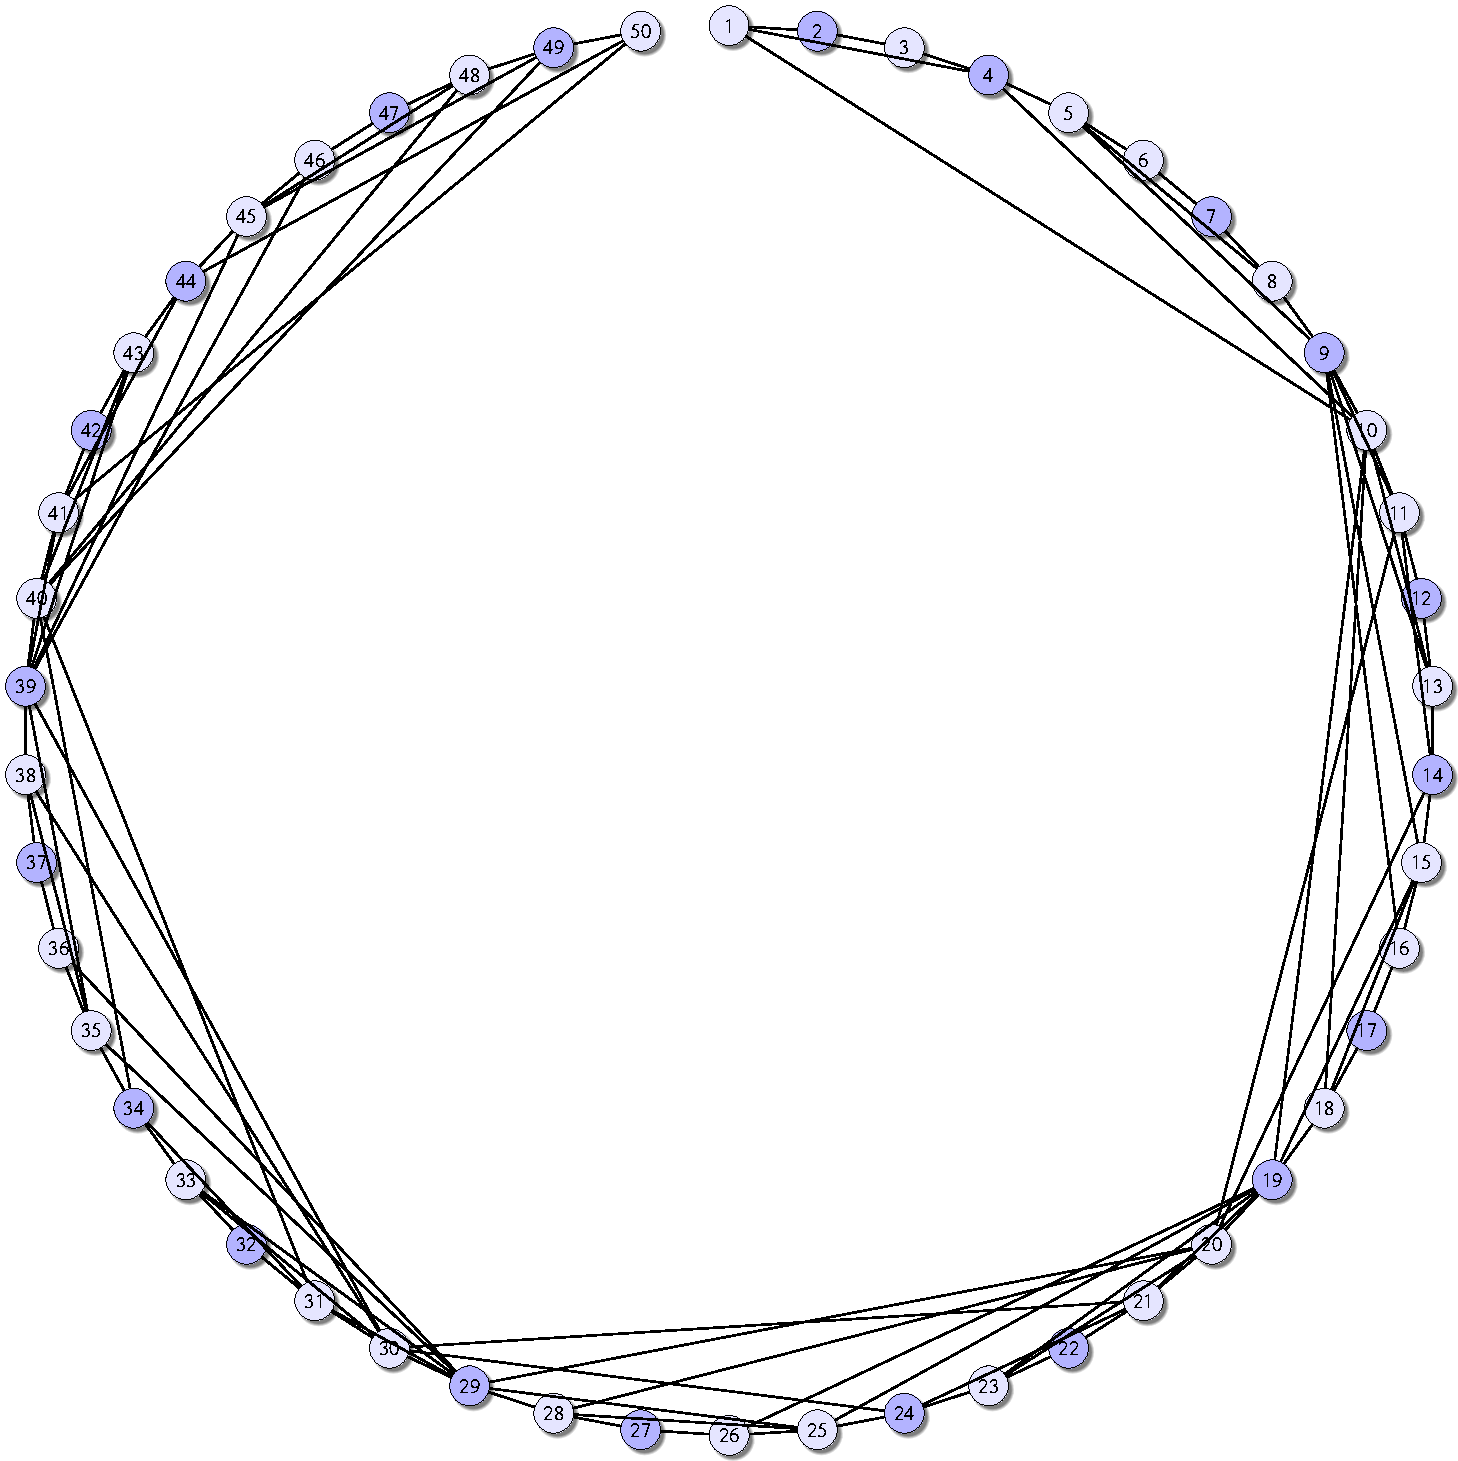
\includegraphics[width=\textwidth]{figures/graph_050.pdf}
  \caption{The graph $G_{5}$ with 50 nodes.}
\end{figure}

\begin{figure}[ht]
  \centering
  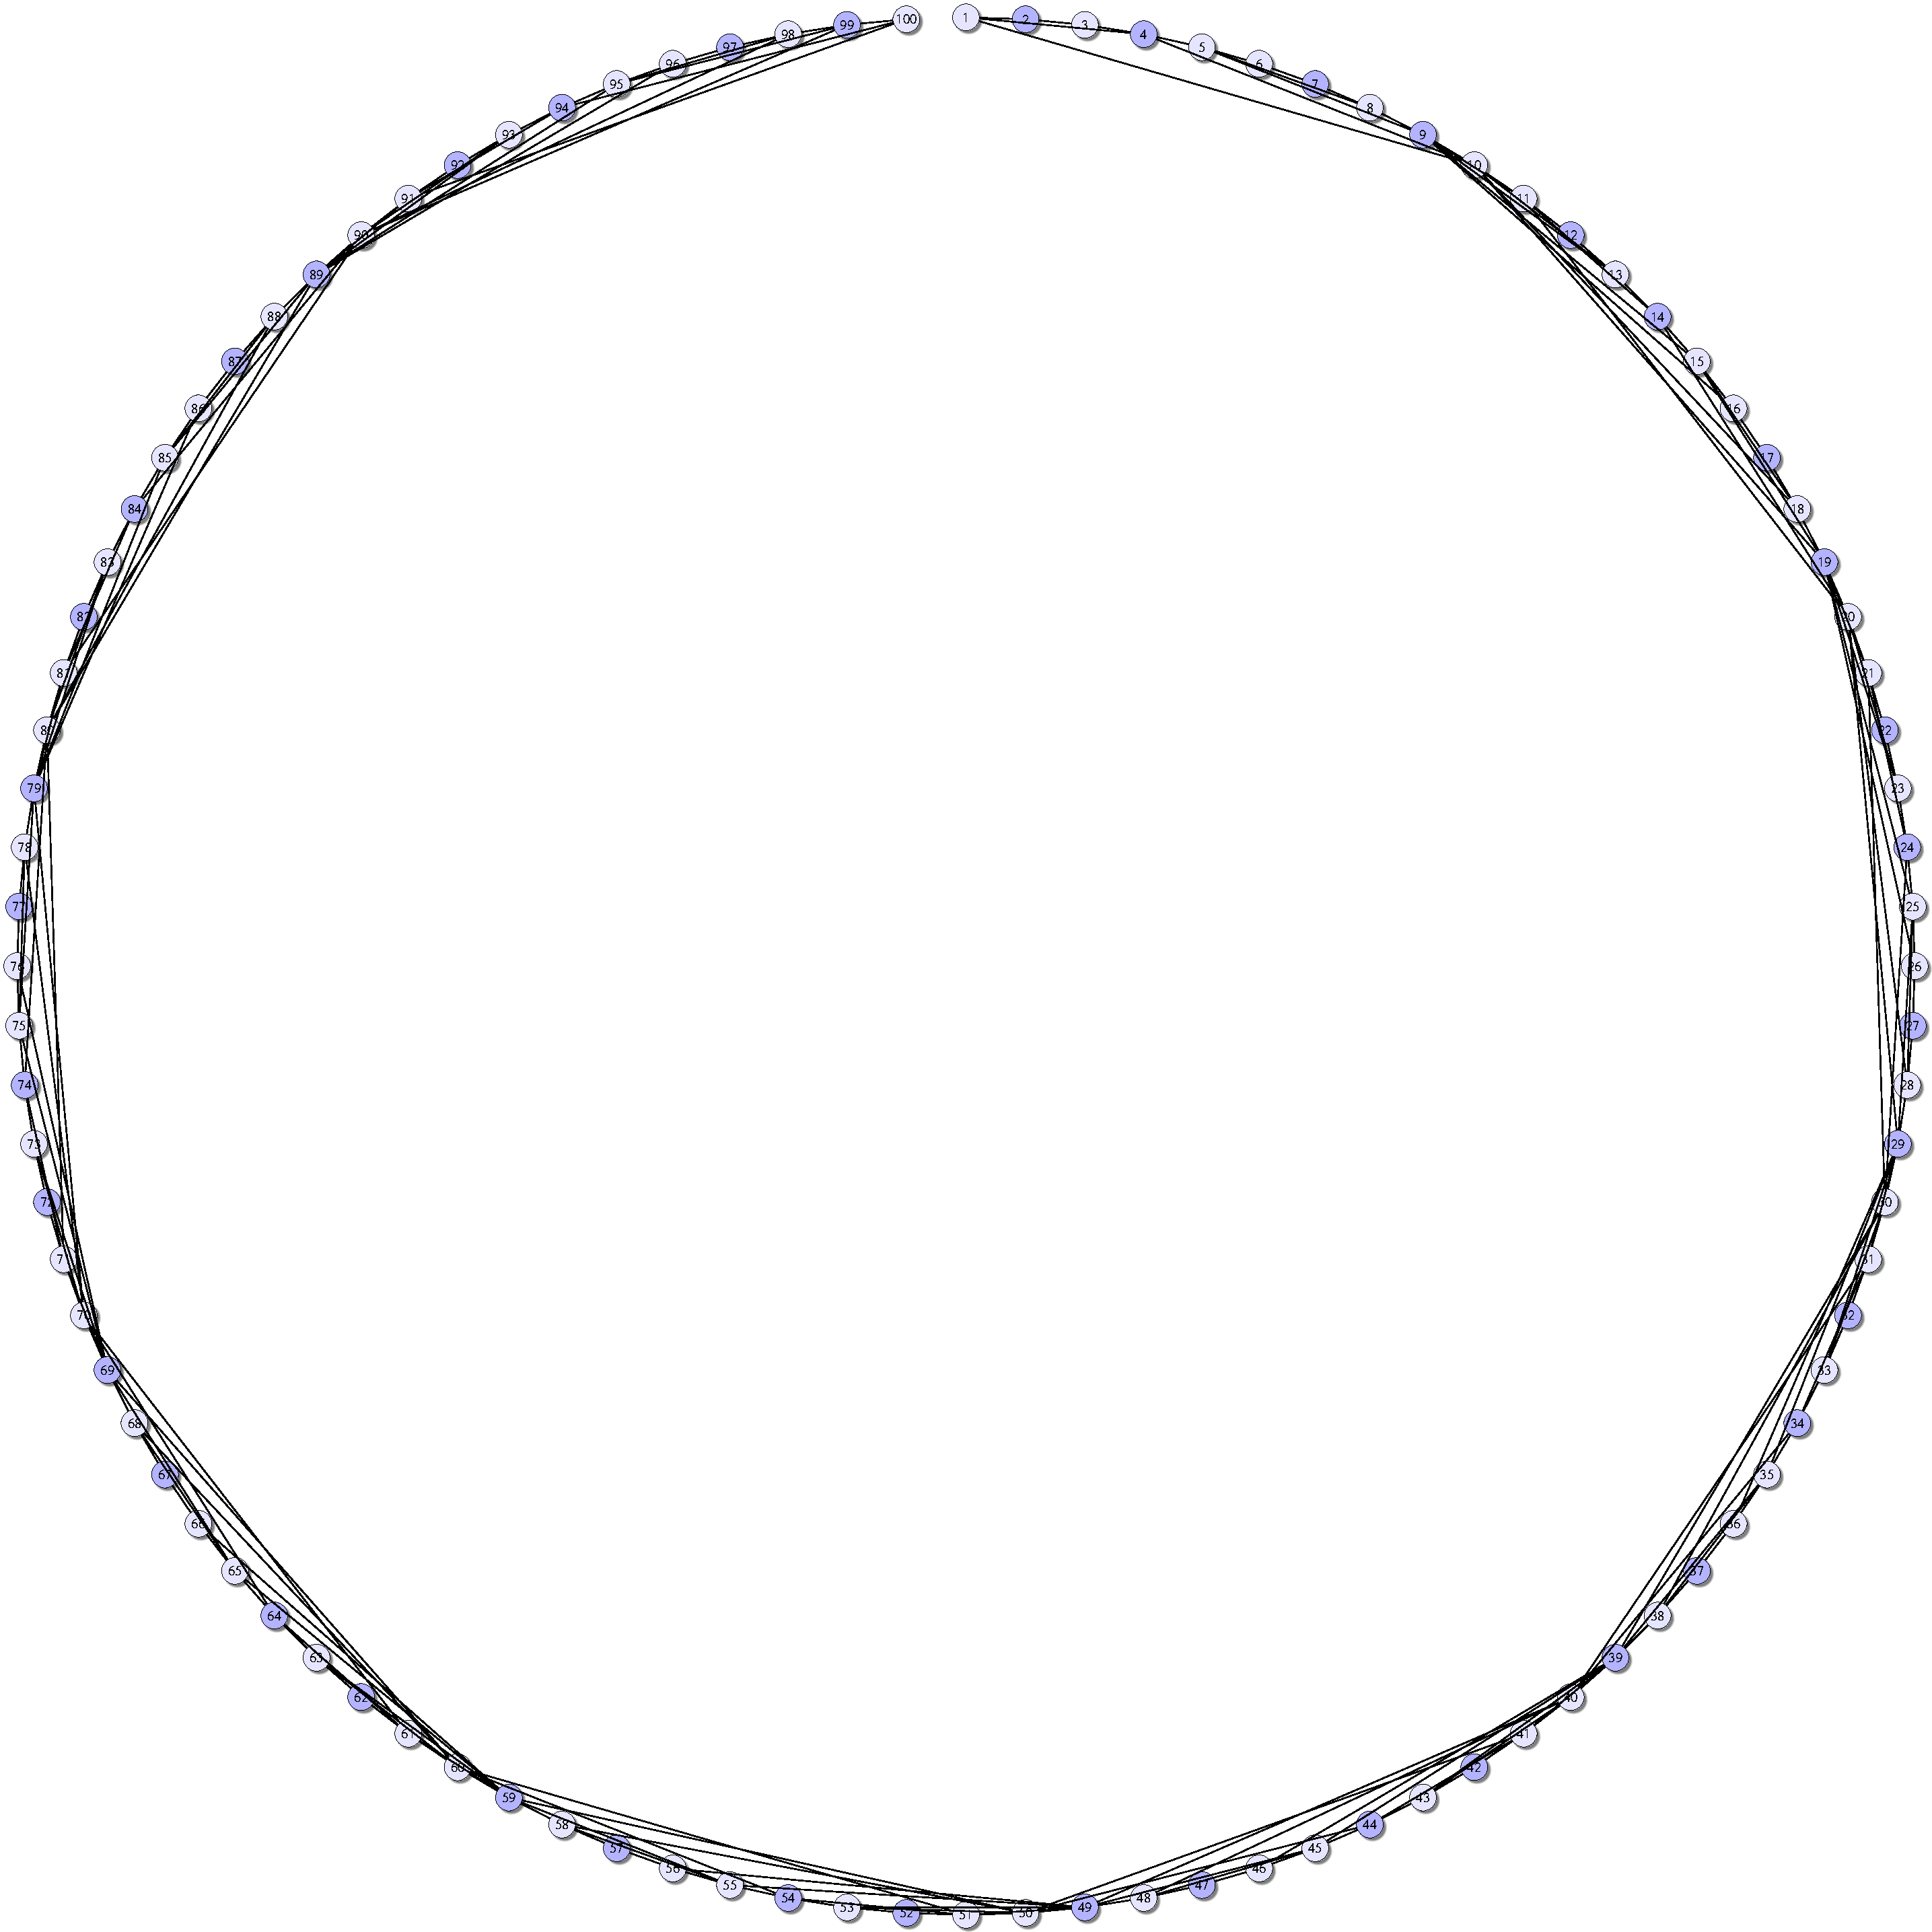
\includegraphics[width=\textwidth]{figures/graph_100.pdf}
  \caption{The graph $G_{10}$ with 100 nodes.}
\end{figure}

\end{document}
